\documentclass[14pt,aspectratio=169]{beamer}
\usepackage[utf8]{inputenc}
\usepackage{wasysym}
\usepackage{svg}
\usepackage{amsmath}
\usepackage{amssymb}
\usepackage{fourier}
\usepackage{physics}

\usepackage{minted}
\usemintedstyle{tango}

\usefonttheme{professionalfonts}

\mode<presentation>

\usetheme{Antibes}
\usecolortheme{seagull}

\setbeamertemplate{navigation symbols}{}
\setbeamertemplate{headline}{} % hide navbar
\setbeamertemplate{footline}[frame number]

\title{Scientific Machine Learning \\ Final Project}
\author{Lovnesh Bhardwaj, Laurynas Varnas}
\date{}

\begin{document}

\begin{frame}
	\titlepage
\end{frame}

\begin{frame}[plain]
	\centering
	\usebeamercolor[fg]{title}\usebeamerfont{title}
	Finite Element Method
\end{frame}

\begin{frame}
	\begin{align*}
		\pdv{u}{t} - \divergence \Sigma \grad u + f(u) & = 0   & \text{in } \Omega \times I,          \\
		\mathbf{n} \cdot \grad u                       & = 0   & \text{on } \partial \Omega \times I, \\
		u                                              & = u_0 & \text{in } \Omega \times \{0\},
	\end{align*}
\end{frame}

\begin{frame}
	\begin{align*}
		\frac{U^{n+1} - U^n}{\Delta t} = \divergence \Sigma \grad U^{n+1} - f(U^n).
	\end{align*}
\end{frame}


\begin{frame}{$\Sigma_d = 10$}
	\begin{table}[H]
		\centering
		\begin{tabular}{l|r|ccc}
			$\Delta t$ & $n_e$ & Activation time & M-matrix?     & $u \in [0, 1]$ \\
			\hline
			0.1        & 64    & 28.60           & \textbf{true} & false          \\
			0.1        & 128   & 29.10           & \textbf{true} & false          \\
			0.1        & 256   & 29.20           & \textbf{true} & false          \\
			0.05       & 64    & 26.60           & false         & false          \\
			0.05       & 128   & 27.15           & \textbf{true} & \textbf{true}  \\
			0.05       & 256   & 27.20           & \textbf{true} & \textbf{true}  \\
			0.025      & 64    & 25.60           & false         & false          \\
			0.025      & 128   & 26.10           & \textbf{true} & \textbf{true}  \\
			0.025      & 256   & 26.175          & \textbf{true} & \textbf{true}  \\
		\end{tabular}
	\end{table}
\end{frame}

\begin{frame}{$\Sigma_d = 1$}
	\begin{table}[H]
		\centering
		\begin{tabular}{l|r|ccc}
			$\Delta t$ & $n_e$ & Activation time & M-matrix?     & $u \in [0, 1]$ \\
			\hline
			0.1        & 64    & 30.20           & \textbf{true} & false          \\
			0.1        & 128   & 30.90           & \textbf{true} & false          \\
			0.1        & 256   & 31.00           & \textbf{true} & false          \\
			0.05       & 64    & 28.10           & false         & false          \\
			0.05       & 128   & 28.80           & \textbf{true} & \textbf{true}  \\
			0.05       & 256   & 28.90           & \textbf{true} & \textbf{true}  \\
			0.025      & 64    & 27.025          & false         & false          \\
			0.025      & 128   & 27.70           & \textbf{true} & \textbf{true}  \\
			0.025      & 256   & 27.775          & \textbf{true} & \textbf{true}  \\
		\end{tabular}
	\end{table}
\end{frame}

\begin{frame}{$\Sigma_d = 0.1$}
	\begin{table}[H]
		\centering
		\begin{tabular}{l|r|ccc}
			$\Delta t$ & $n_e$ & Activation time & M-matrix?     & $u \in [0, 1]$ \\
			\hline
			0.1        & 64    & 31.70           & false         & false          \\
			0.1        & 128   & 32.50           & false         & false          \\
			0.1        & 256   & 32.60           & \textbf{true} & false          \\
			0.05       & 64    & 29.55           & false         & false          \\
			0.05       & 128   & 30.25           & false         & false          \\
			0.05       & 256   & 30.40           & false         & \textbf{true}  \\
			0.025      & 64    & 28.40           & false         & false          \\
			0.025      & 128   & 29.075          & false         & false          \\
			0.025      & 256   & 29.225          & false         & \textbf{true}  \\
		\end{tabular}
	\end{table}
\end{frame}

\begin{frame}
\end{frame}

\begin{frame}
	\centering
	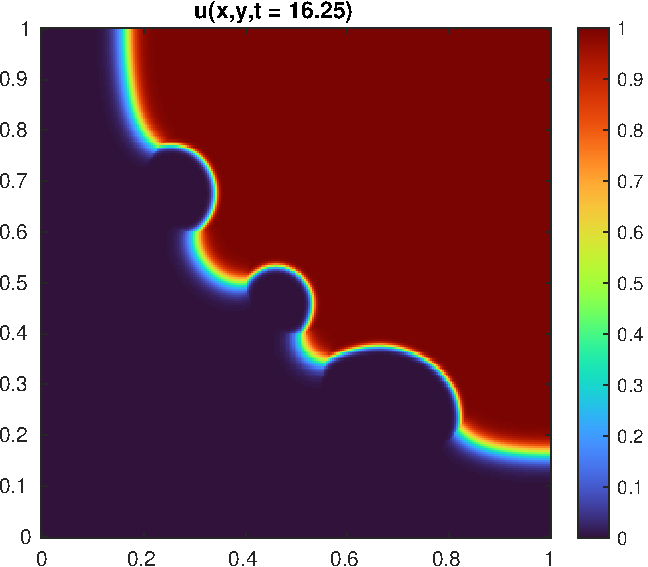
\includegraphics[height=\textheight]{figs/S01.pdf}
\end{frame}

\begin{frame}
	\centering
	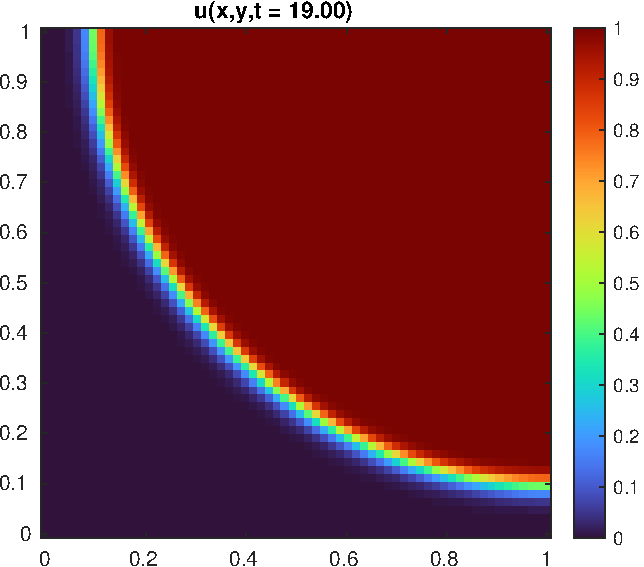
\includegraphics[height=\textheight]{figs/S1.pdf}
\end{frame}

\begin{frame}
	\centering
	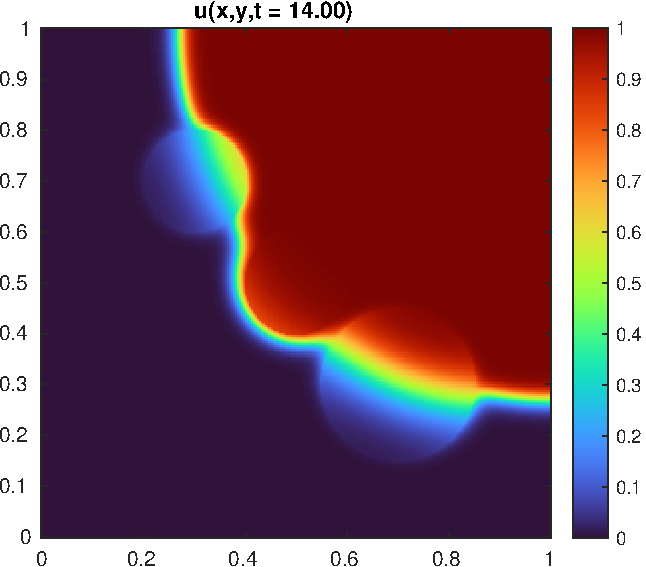
\includegraphics[height=\textheight]{figs/S10.pdf}
\end{frame}

% \begin{frame}{GCN}
% 	\centering
% 	\includegraphics[width=\textwidth]{./img/batched_plots.pdf}
% \end{frame}
%
% \begin{frame}{GCN with gradient accumulation}
% 	\centering
% 	\includegraphics[width=\textwidth]{./img/acc_plots.pdf}
% \end{frame}
%
% % \begin{frame}{Benchmark Code}
% % 	\centering
% % 	\includegraphics[width=.7\textwidth]{./img/loss_plots.pdf}
% % \end{frame}
%
%
% \begin{frame}{GCN Layer}
%
% 	\begin{equation*}
% 		H^{(l+1)} = \sigma\left( D^{-1/2} \tilde{A} D^{-1/2} H^{(l)} W^{(l)} \right)
% 	\end{equation*}
%
% 	\begin{itemize}
% 		% \item \(H^{(l)}\): Node feature matrix at layer \(l\).
% 		% \item \(\tilde{A} = A + I\): Adjacency matrix with self-loops added.
% 		% \item \(D\): Degree matrix (\( D_{ii} = \sum_j \tilde{A}_{ij} \)).
% 		% \item \(W^{(l)}\): Learnable weight matrix at layer \(l\).
% 		% \item \(\sigma\): Activation function (ReLU).
% 		\item $\tilde{A} = A + I$, $\tilde{A} \in \mathbb{R}^{n \times n}$: adjacency matrix with self-loops.
% 		\item $D \in \mathbb{R}^{n \times n}$: degree matrix ($D_{ii} = \sum_j \tilde{A}_{ij}$).
% 		\item $H^{(l)} \in \mathbb{R}^{n \times d}$: input - per-node feature vectors at layer \(l\).
% 		\item $W^{(l)} \in \mathbb{R}^{d \times w}$: layer $l$ weights.
% 		\item \(\sigma\): activation function (ReLU).
% 	\end{itemize}
% \end{frame}
%
%
% \begin{frame}[fragile]\frametitle{GCN input}
% 	\begin{verbatim}
% x = torch.Size([3766, 3])
% tensor([[0.2539, 0.2363, 0.2412],
%         [0.3328, 0.2896, 0.3184],
%         [0.3301, 0.2183, 0.3960],
%         ...,
%         [0.6509, 0.6431, 0.6611],
%         [0.6768, 0.6768, 0.6772],
%         [0.5552, 0.4404, 0.4204]])
% \end{verbatim}
% \end{frame}

% \begin{frame}{Adam}
%
% 	% \[
% 	% 	\text{Given: } \theta_t \text{ (parameters)}, \alpha \text{ (learning rate)}, \beta_1, \beta_2 \text{ (moment decay rates)}, \epsilon \text{ (small constant)}.
% 	% \]
%
% 	% \textbf{Initialization: }
% 	% \[
% 	% 	m_0 = 0, \quad v_0 = 0, \quad t = 0.
% 	% \]
%
% 	\textbf{For each timestep } \( t \):
% 	\[
% 		\begin{aligned}
% 			1. \quad & t \leftarrow t + 1,                                                                     \\
% 			2. \quad & g_t = \nabla_{\theta} f(\theta_{t-1}) + \lambda \theta_{t-1} \text{ --- weight decay} , \\
% 			3. \quad & m_t = \beta_1 m_{t-1} + (1 - \beta_1) g_t,                                              \\
% 			4. \quad & v_t = \beta_2 v_{t-1} + (1 - \beta_2) g_t^2,                                            \\
% 			5. \quad & \hat{m}_t = \frac{m_t}{1 - \beta_1^t},                                                  \\
% 			6. \quad & \hat{v}_t = \frac{v_t}{1 - \beta_2^t},                                                  \\
% 			7. \quad & \theta_t = \theta_{t-1} - \alpha \frac{\hat{m}_t}{\sqrt{\hat{v}_t} + \epsilon}.
% 		\end{aligned}
% 	\]
%
% \end{frame}

\end{document}
